\documentclass[12pt,a4paper]{article}


\usepackage[in, plain]{fullpage}
\usepackage{array}
\usepackage{../../../pas-math}

%-------------------------------------------------------------------------------
%          -Packages nécessaires pour écrire en Français et en UTF8-
%-------------------------------------------------------------------------------
\usepackage[utf8]{inputenc}
\usepackage[frenchb]{babel}
\usepackage[T1]{fontenc}
\usepackage{lmodern}
\usepackage{textcomp}



%-------------------------------------------------------------------------------

%-------------------------------------------------------------------------------
%                          -Outils de mise en forme-
%-------------------------------------------------------------------------------
\usepackage{hyperref}
\hypersetup{pdfstartview=XYZ}
%\usepackage{enumerate}
\usepackage{graphicx}
\usepackage{multicol}
\usepackage{tabularx}
\usepackage{multirow}


\usepackage{anysize} %%pour pouvoir mettre les marges qu'on veut
%\marginsize{2.5cm}{2.5cm}{2.5cm}{2.5cm}

\usepackage{indentfirst} %%pour que les premier paragraphes soient aussi indentés
\usepackage{verbatim}
\usepackage{enumitem}
\usepackage[usenames,dvipsnames,svgnames,table]{xcolor}

\usepackage{variations}

%-------------------------------------------------------------------------------


%-------------------------------------------------------------------------------
%                  -Nécessaires pour écrire des mathématiques-
%-------------------------------------------------------------------------------
\usepackage{amsfonts}
\usepackage{amssymb}
\usepackage{amsmath}
\usepackage{amsthm}
\usepackage{tikz}
\usepackage{xlop}
%-------------------------------------------------------------------------------



%-------------------------------------------------------------------------------


%-------------------------------------------------------------------------------
%                    - Mise en forme avancée
%-------------------------------------------------------------------------------

\usepackage{ifthen}
\usepackage{ifmtarg}


\newcommand{\ifTrue}[2]{\ifthenelse{\equal{#1}{true}}{#2}{$\qquad \qquad$}}

%-------------------------------------------------------------------------------

%-------------------------------------------------------------------------------
%                     -Mise en forme d'exercices-
%-------------------------------------------------------------------------------
%\newtheoremstyle{exostyle}
%{\topsep}% espace avant
%{\topsep}% espace apres
%{}% Police utilisee par le style de thm
%{}% Indentation (vide = aucune, \parindent = indentation paragraphe)
%{\bfseries}% Police du titre de thm
%{.}% Signe de ponctuation apres le titre du thm
%{ }% Espace apres le titre du thm (\newline = linebreak)
%{\thmname{#1}\thmnumber{ #2}\thmnote{. \normalfont{\textit{#3}}}}% composants du titre du thm : \thmname = nom du thm, \thmnumber = numéro du thm, \thmnote = sous-titre du thm

%\theoremstyle{exostyle}
%\newtheorem{exercice}{Exercice}
%
%\newenvironment{questions}{
%\begin{enumerate}[\hspace{12pt}\bfseries\itshape a.]}{\end{enumerate}
%} %mettre un 1 à la place du a si on veut des numéros au lieu de lettres pour les questions 
%-------------------------------------------------------------------------------

%-------------------------------------------------------------------------------
%                    - Mise en forme de tableaux -
%-------------------------------------------------------------------------------

\renewcommand{\arraystretch}{1.7}

\setlength{\tabcolsep}{1.2cm}

%-------------------------------------------------------------------------------



%-------------------------------------------------------------------------------
%                    - Racourcis d'écriture -
%-------------------------------------------------------------------------------

% Angles orientés (couples de vecteurs)
\newcommand{\aopp}[2]{(\vec{#1}, \vec{#2})} %Les deuc vecteurs sont positifs
\newcommand{\aopn}[2]{(\vec{#1}, -\vec{#2})} %Le second vecteur est négatif
\newcommand{\aonp}[2]{(-\vec{#1}, \vec{#2})} %Le premier vecteur est négatif
\newcommand{\aonn}[2]{(-\vec{#1}, -\vec{#2})} %Les deux vecteurs sont négatifs

%Ensembles mathématiques
\newcommand{\naturels}{\mathbb{N}} %Nombres naturels
\newcommand{\relatifs}{\mathbb{Z}} %Nombres relatifs
\newcommand{\rationnels}{\mathbb{Q}} %Nombres rationnels
\newcommand{\reels}{\mathbb{R}} %Nombres réels
\newcommand{\complexes}{\mathbb{C}} %Nombres complexes


%Intégration des parenthèses aux cosinus
\newcommand{\cosP}[1]{\cos\left(#1\right)}
\newcommand{\sinP}[1]{\sin\left(#1\right)}


%Probas stats
\newcommand{\stat}{statistique}
\newcommand{\stats}{statistiques}
%-------------------------------------------------------------------------------

%-------------------------------------------------------------------------------
%                    - Mise en page -
%-------------------------------------------------------------------------------

\newcommand{\twoCol}[1]{\begin{multicols}{2}#1\end{multicols}}


\setenumerate[1]{font=\bfseries,label=\textit{\alph*})}
\setenumerate[2]{font=\bfseries,label=\arabic*)}


%-------------------------------------------------------------------------------
%                    - Elements cours -
%-------------------------------------------------------------------------------




\title{Correction des exercices bonus de calcul littéral}
\date{}

\begin{document}
	
\maketitle

\vspace*{-1cm}

\section*{Exercice 58}


\begin{enumerate}[label={\arabic*)}]
	
%	\begin{multicols}{2}
		
		
		
		
	
	\item \begin{enumerate}[label={\alph*)}]
		\item \ 
		\begin{center}
			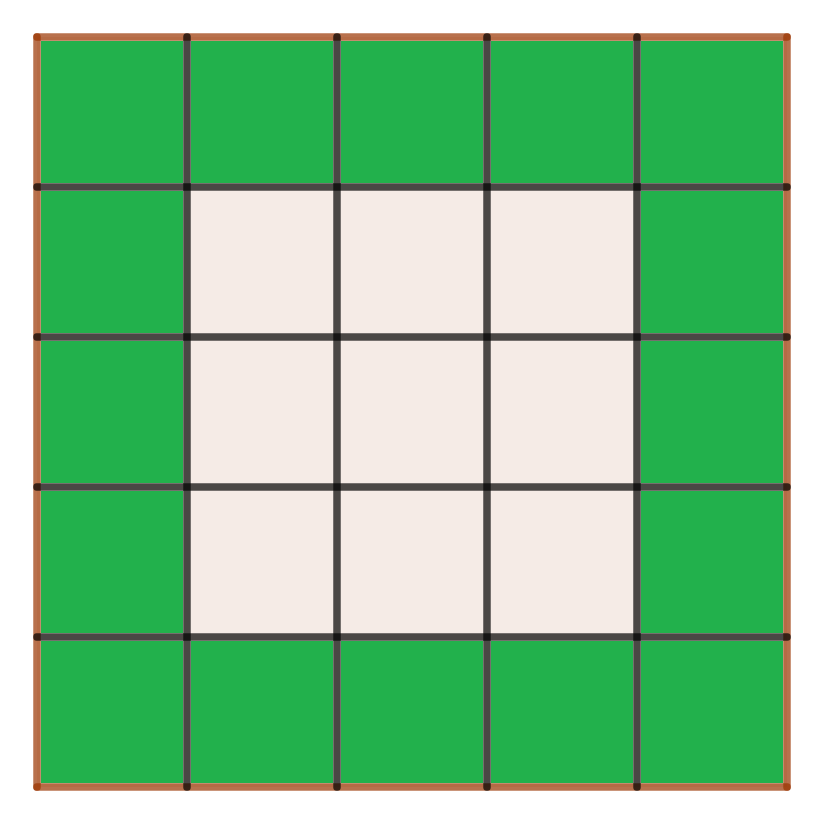
\includegraphics[scale=0.2]{./img/carre}
		\end{center}
	
		\item Pour construire ce carré, il faut 16 carrés verts.
	\end{enumerate}
	
	
	\item \begin{enumerate}[label={\alph*)}]
		\item Sur la figure on voit que chaque rectangle vert s'arrête un carreau avant la fin du côté. Il a pu écrire l'expression :
		
		\begin{equation*}
			4(n-1)
		\end{equation*}
	
		\item Garance a dans un premier temps calculé le nombre total de carreaux de la figure ($n^2$) puis elle a enlevé le carré intérieur ($(n-2)^2$).
		
		\item On pose $n=123$ :
		
		\begin{multicols}{2}
			\begin{align*}
				A &= 4(n-1) \\
				A &= 4 \times (123 - 1)\\
				A &= 4 \times 122 \\
				A &= 488 \\
			\end{align*}
			
			\begin{align*}
				B &= n^2 - (n-2)^2 \\
				B &= 123^2 - (123-2)^2 \\
				B &= 123^2 - (121)^2 \\
				B &= \num{15129} - \num{14641} \\
				B &= 488
			\end{align*}
		\end{multicols}

		Oui ils trouvent le même nombre de carreaux verts pour $n=123$, soit 488.
	\end{enumerate}	
\end{enumerate}

\newpage

\section*{Exercice 59}

	\begin{enumerate}[label=\arabic*)]
		\item \begin{enumerate} [label=\alph*)]
			\item Il faut 11 allumettes pour construire 5 triangles.
			\item Il faut 17 allumettes pour construire 8 triangles.
			\item Il faut 23 allumettes pour construire 11 triangles.
			
		\end{enumerate}
	
		\item Pour chaque nouveau triangle on utilise une allumette du précédent puis on en ajoute 2. Pour construire $n$ triangles il faut $1 + 2n$ allumettes.
		
		\item On veut construire 100 triangles, on pose donc $n=100$, on a donc :
		
		\begin{align*}
			1 + 2n &= 1 + 2 \times 100 \\
			1 + 2n &= 1 + 200 \\
			1 + 2n &= 201 			
		\end{align*}
		
		\item \begin{enumerate}[label=\alph*)]
			\item Avec 99 allumettes on peut construire 49 triangles.
			\item Avec 900 allumettes on peut construire 99 triangles, il en restera une.
		\end{enumerate}
	\end{enumerate}

\section*{Exercice 83}
	
	\begin{enumerate}[label=\arabic*)]
		\item \begin{enumerate}[label=\alph*)]
			\item \begin{equation*}
				(8 + 15) \div 2 = 23 \div 2 = \num{11.5}
			\end{equation*}
			
			En choisissant 8, elle obtient \num{11.5}.
			
			\item L'expression littérale qui correspond au programme de Jade est :\begin{equation*}
				(x + 15) \div 2
			\end{equation*}
		\end{enumerate}
	
		\item \begin{enumerate}[label=\alph*)]
			\item \begin{equation*}
				(9 + 15) \div 2 = 12
			\end{equation*} 
			
			Pour trouver 12 elle a choisi le nombre 9.
			
			
			\item L'expression littérale pour retrouver le nombre de départ à partir du nombre obtenu est :
			
				\begin{equation*}
					y \times 2 - 15
				\end{equation*}
		\end{enumerate}
		
		
		
		
		
	\end{enumerate}


	\section*{Exercice 89}
	
		\begin{multicols}{3}
			
			\begin{enumerate}
				\item \begin{align*}
					3x \times 2 &= 3 \times x \times 2 \\
					3x \times 2 &= 3 \times 2 \times x \\
	%				3x \times 2 &= 6 \times x \\
					3x \times 2 &= 6x 
				\end{align*}
				
				
				\item \begin{align*}
%					&\\
					3x +2 &= 3x +2\\
				\end{align*}
				
				\item \begin{align*}
%					&\\
					3x -2 &= 3x -2\\
				\end{align*}
				
				\item \begin{align*}
					3x \times 2x &= 3 \times x \times 2 \times x\\
					3x \times 2x &= 3 \times 2 \times x \times x \\
					3x \times 2x &= 6x^2 
				\end{align*}
				
				\item \begin{align*}
					3x \div 2 &= 3 \times x \div 2 \\
					3x \div 2 &= 3 \div 2 \times x \\
					%				3x \times 2 &= 6 \times x \\
					3x \div 2 &= \num{1.5}x 
				\end{align*}
				
				
				\item \begin{align*}
					3x + 2x &= (3 + 2) \times x\\
					3x + 2x &= 5 \times x\\
				\end{align*}
			\end{enumerate}
		
		\end{multicols}
	
\section*{Exercice 90}

	\begin{enumerate}[label=\arabic*)]
		\item 
	
	\begin{enumerate}[label=\alph*)]
		\item Soit $x=4$
		
		\begin{multicols}{2}
			\begin{align*}
				(x + 6)^2 &= (4 + 6)^2\\ 
				(x + 6)^2 &= 10^2\\ 
				(x + 6)^2 &= 100
			\end{align*}
			
			\begin{align*}
				25x &= 25 \times 4\\ 
				25x &= 100\\
			\end{align*}
		\end{multicols}
		
		L'égalité est vraie pour $x=4$.
		\item Soit $x=7$
		
		\begin{multicols}{2}
			\begin{align*}
				(x + 6)^2 &= (7 + 6)^2\\ 
				(x + 6)^2 &= 13^2\\ 
				(x + 6)^2 &= 169
			\end{align*}
			
			\begin{align*}
				25x &= 25 \times 7\\ 
				25x &= 175\\
			\end{align*}
		\end{multicols}
		
		L'égalité est fausse pour $x=7$.
		\item Soit $x=9$
		
		\begin{multicols}{2}
			\begin{align*}
				(x + 6)^2 &= (9 + 6)^2\\ 
				(x + 6)^2 &= 15^2\\ 
				(x + 6)^2 &= 225
			\end{align*}
			
			\begin{align*}
				25x &= 25 \times 9\\ 
				25x &= 225\\
			\end{align*}
		\end{multicols}
	
		L'égalité est vraie pour $x=9$.
		\item Soit $x=10$
		
		\begin{multicols}{2}
			\begin{align*}
				(x + 6)^2 &= (10 + 6)^2\\ 
				(x + 6)^2 &= 16^2\\ 
				(x + 6)^2 &= 256
			\end{align*}
			
			\begin{align*}
				25x &= 25 \times 10\\ 
				25x &= 250\\
			\end{align*}
		\end{multicols}
	
		L'égalité est fausse pour $x=10$.
	\end{enumerate}
	
	\item La mesure des côtés du carré est $x+6$ donc son aire est $(x+6)\times (x+6)$, soit $(x+6)^2$. La largeur du rectangle vaut $x$ et sa Longueur 25, donc son aire est $25 \times x$ soit $25x$. J'en déduis que le rectangle et le carré ont la même aire pour $x=4$ et $x=9$.
	\end{enumerate}
\end{document}